	% Set document type and scheme
	\documentclass[10pt]{beamer}
	\usetheme[progressbar=frametitle]{metropolis}
	\usepackage{lmodern}

	% Load packages
	\usepackage{appendixnumberbeamer}
	\usepackage{booktabs}
	\usepackage[scale=2]{ccicons}
	\usepackage{pgfplots}
	\usepackage{xspace}
		\newcommand{\themename}{\textbf{\textsc{metropolis}}\xspace}
	\usepackage{stata}


	\title{Stata Workshop} %% that will be typeset on the
	\subtitle{At MINAGRI} %% title page.
	\author{Roshni Khincha and Sakina Shibuya \\ DIME, World Bank}
	\date{August, 2018}

	\titlegraphic{%
		
\includegraphics[width=.2\textwidth]{DIME}\hfill % I think I should probably ask for a better image for this thing....
		
\includegraphics[width=.15\textwidth]{logo_minagri}\hfill
		
\includegraphics[width=.2\textwidth]{logo_eu}
		}

	\makeatletter
	\setbeamertemplate{title page}{
		\begin{minipage}[b][\paperheight]{\textwidth}
			\vfill%
			\ifx\inserttitle\@empty\else\usebeamertemplate*{title}\fi
			\ifx\insertsubtitle\@empty\else\usebeamertemplate*{subtitle}\fi
			\usebeamertemplate*{title separator}
			\ifx\beamer@shortauthor\@empty\else\usebeamertemplate*{author}\fi
			\ifx\insertdate\@empty\else\usebeamertemplate*{date}\fi
			\vfill
			\ifx\inserttitlegraphic\@empty\else\inserttitlegraphic\fi
			\vspace*{1cm}
		\end{minipage}
		}
	\makeatother

	\begin{document}
		
	\maketitle

	\section{Section 1}
	\section{Section 2}

	\begin{frame}
	\frametitle{\textsc{Edit data in Stata}}
\begin{stlog}tabulate s5bq3a
summarize s5bq3a 
codebook s5bq3a
\end{stlog}
	\end{frame}
	
	\begin{frame}
	\frametitle{\textsc{Lab Task 7: Saving Stata datasets}}	
		\begin{itemize}
			\item The command for saving a Stata dataset is \textit{\textbf{save}}.
			\item \textit{save} saves your data in memory in a file format called dta. This is a file that can only be read with Stata.
			\item The command for saving a dataset in excel and csv is \textit{\textbf{export}}.
			\item \textit{\textbf{export}} is the opposite of import, and is very versatile. 
				  It lets you save data in excel, csv, sas and others. 
				  Please refer to the help file on \textit{\textbf{export}}.
		\end{itemize}	
	\end{frame}

	\begin{frame}
	\frametitle{\textsc{Lab Task 7: Saving Stata datasets}}	
		\begin{columns}
			\begin{column}{0.5\textwidth}
				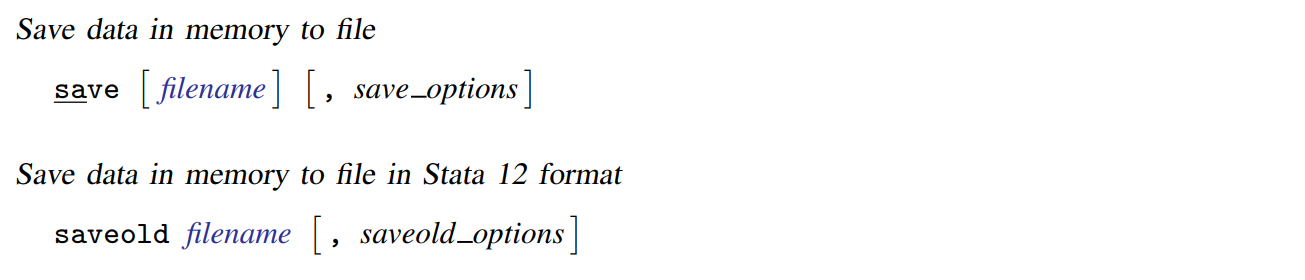
\includegraphics[width=\linewidth]{helpfile_save_1}
				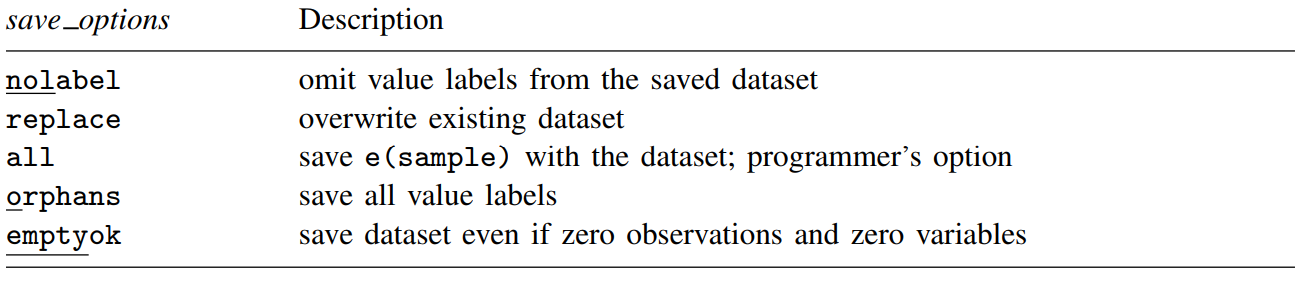
\includegraphics[width=\linewidth]{helpfile_save_2}
			\end{column}
			\begin{column}{0.5\textwidth}
				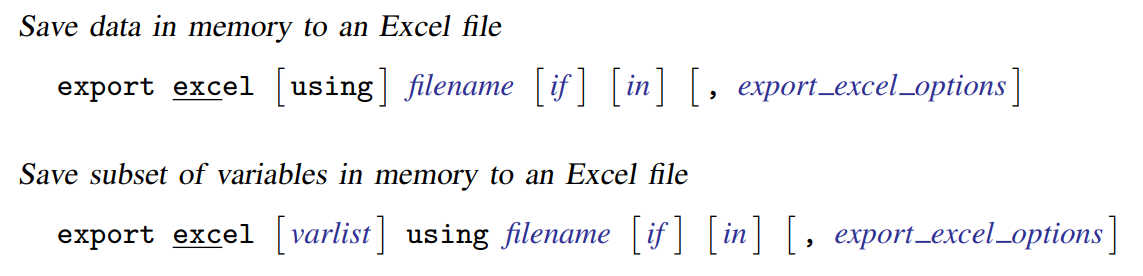
\includegraphics[width=\linewidth]{helpfile_exportexcel_1}
				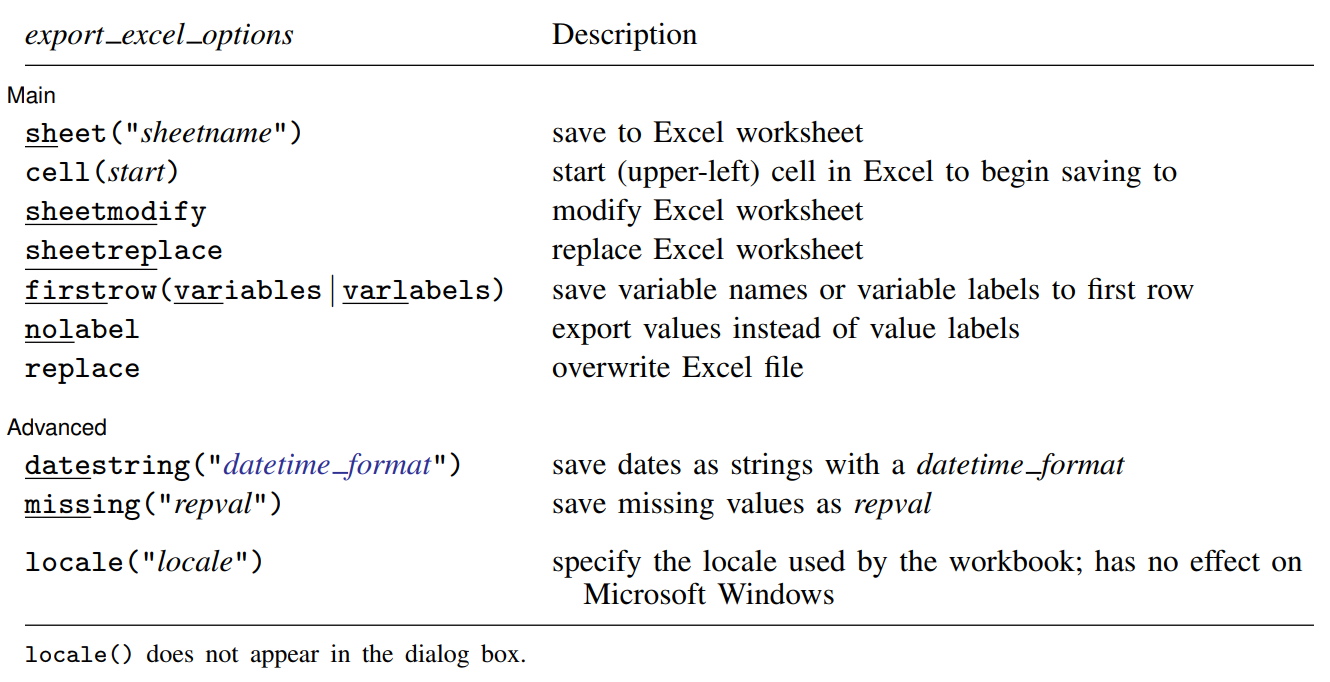
\includegraphics[width=\linewidth]{helpfile_exportexcel_2}
			\end{column}
		\end{columns}
	\end{frame}
	
	\begin{frame}
		\frametitle{\textsc{Lab Task 7: Saving Stata datasets}}	
		\onslide<1-> Let's save the modified data as a dta file.
					\vspace{2mm} Type...
\begin{stlog}. tabulate ur2012 
\end{stlog}
		\vspace{2mm}
		\onslide<2-> Notice that we use the \textbf{\textit{replace}} option. 
					 This overwrites the existing file. 
					 \vspace{2mm} Type the same command without \textbf{\textit{, replace}}, 
					 and see what error you get! 
		\vspace{2mm}			 
		\onslide<3-> Did you get an error like this? 
		\begin{centering}			
			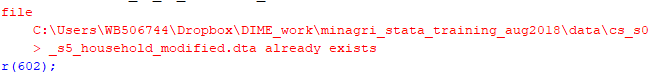
\includegraphics[width=0.8\linewidth]{error_save_existing}
		\end{centering}
	\end{frame}
	
	\begin{frame}
		\frametitle{\textsc{Lab Task 7: Saving Stata datasets}}
		\onslide<1-> Now, let's save the modified data as a excel. 
					 This is helpful if you are sending the dataset to 
					 someone who does not use or have Stata. \\
					 Type...
		\vspace{2mm}
\begin{stlog}. use "$data\\cs_s0_s5_household.dta", clear
{\smallskip}
\end{stlog}
		\vspace{2mm}
		\onslide<2-> Open the output file. 
					 Notice that it doesn't have variable names as column names.
					 This is very inconvenient!
		\onslide<3-> Use an optional command, \textbf{\textit{firstrow(variables)}}.
		\vspace{2mm}
\begin{stlog}. keep hhid province district ur2012 s5cq2 s5cq4 s5cq8 s5cq15 s5cq23 s5bq2 s5cq22 s5cq1
> 3 s5cq17 
{\smallskip}
\end{stlog}
		\vspace{2mm}
		\onslide<4-> Open the newly saved excel file. You will find column names!
	\end{frame}
	
	
	\section{Section 3: Introduction to Stata Grphics}
	
	\begin{frame}
	\frametitle{Placer}
	Add the first several pages from the FC training on data visualization.
	\end{frame}
	
	\begin{frame}
	\frametitle{\textsc{Box plot}}
		\onslide<1-> Let's make a a box plot like the one below 
					 using the drop down menu first.
\begin{center}
    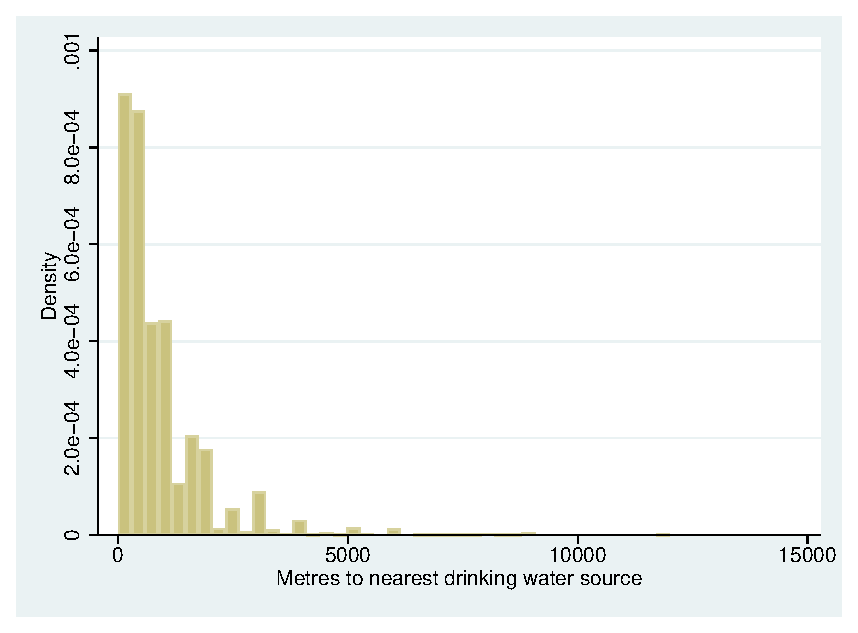
\includegraphics[width=0.8\textwidth]{stata_workshop_for_govt_officials_4.eps}
\end{center}
	\end{frame}
	
	\begin{frame}
	\frametitle{\textsc{Box plot}}	
		\begin{enumerate}
			\onslide<1-> \item Click Graphics on the top left side, and select \textit{Box plot}.
			\vspace{2mm} 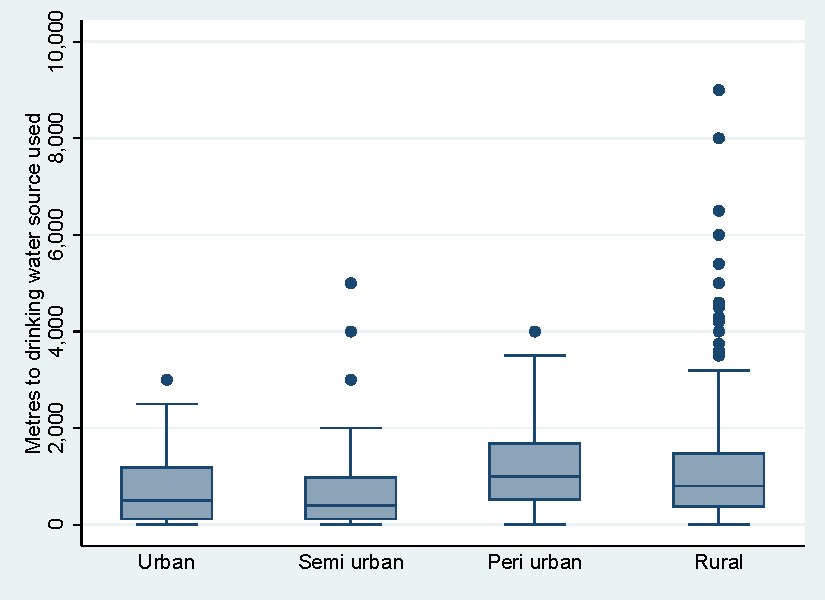
\includegraphics[width=0.5\linewidth]{boxplot_1}
			\onslide<2-> \item In the \textit{Main} tab, select the variable \textit{m\_drink\_ws}.
			\onslide<3-> \item In the \textit{Categories} tab, select \textit{Group 1} and \textit{urban\_2012} as your grouping variable.
			\onslide<4-> \item Then, press ok.
		\end{enumerate}
	\end{frame}

	
	\begin{frame}
	\frametitle{\textsc{Histogram}}
\begin{center}
    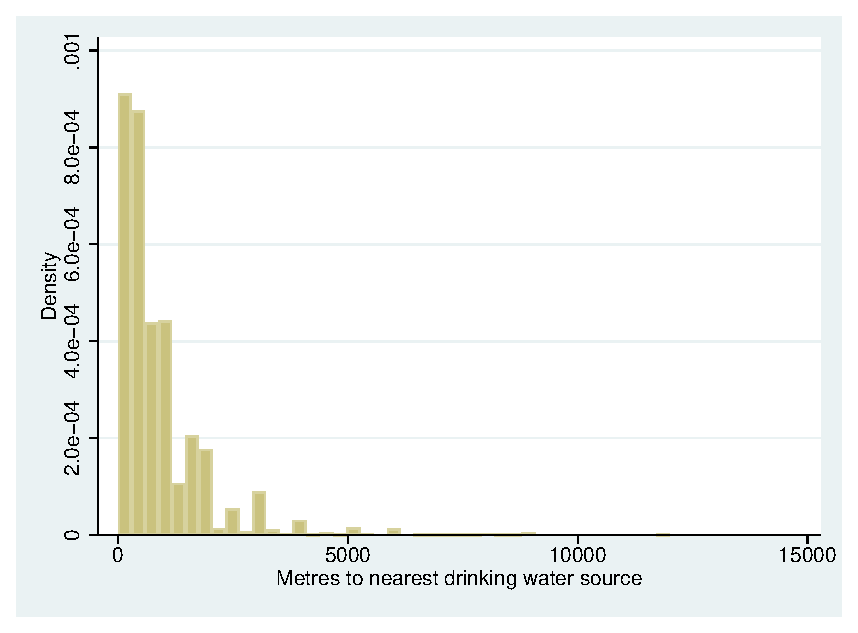
\includegraphics[width=0.8\textwidth]{stata_workshop_for_govt_officials_4.eps}
\end{center}
	\end{frame}
	
	\begin{frame}
	\frametitle{\textsc{Oneway graphs}}
	blah blah
	\end{frame}

	\begin{frame}
	\frametitle{\textsc{Twoway graphs}}
	blah blah
	\end{frame}
	
	\begin{frame}
	\frametitle{\textsc{Saving and combining graphs}}
	blah blah
	\end{frame}



	\end{document}
